% !TEX root = main.tex
\documentclass[12pt,a4paper]{ltjsarticle}

%% Fonts
\usepackage{lmodern}
\usepackage{luatexja-preset}

%% Layout
\usepackage[top=30mm, bottom=25mm, left=25mm, right=25mm]{geometry}

%% Color / graphics
\usepackage[svgnames,table]{xcolor}
\usepackage{graphicx}

%% Diagrams / charts
\usepackage{tikz}
\usepackage{pgfplots}
\pgfplotsset{compat=1.18}

%% Source code listings
\usepackage{listings}
\renewcommand{\lstlistingname}{ソースコード}

%% Hyperlinks (load near last)
\usepackage{hyperref}

%% Header / footer
\usepackage{fancyhdr}

%% Captions
\usepackage[format=hang, font=small, labelfont=bf]{caption}
\usepackage{subcaption}

%% Mathematics
\usepackage{amsmath}
\usepackage{amssymb}

%% Professional table rules
\usepackage{booktabs}

%% URL
\usepackage{url}

%% List customization
\usepackage{enumitem}
\setlist{topsep=2pt, partopsep=0pt}

%% ── Section Numbering ────────────────────────────────────────
\renewcommand{\thesection}{\arabic{section}.}
\renewcommand{\thesubsection}{\arabic{section}.\arabic{subsection}}
\renewcommand{\thesubsubsection}{\arabic{section}.\arabic{subsection}.\arabic{subsubsection}}

%% ── Source Code Appearance ───────────────────────────────────
\definecolor{codebg}{RGB}{248,248,248}
\definecolor{codeframe}{RGB}{180,180,180}
\definecolor{kwcolor}{RGB}{0,0,180}
\definecolor{cmcolor}{RGB}{100,100,100}
\definecolor{stcolor}{RGB}{160,0,0}

\lstset{
  backgroundcolor  = \color{codebg},
  basicstyle       = \ttfamily\small,
  keywordstyle     = \color{kwcolor}\bfseries,
  commentstyle     = \color{cmcolor}\itshape,
  stringstyle      = \color{stcolor},
  numbers          = left,
  numberstyle      = \tiny\color{gray},
  numbersep        = 8pt,
  frame            = single,
  rulecolor        = \color{codeframe},
  breaklines       = true,
  breakatwhitespace= false,
  showstringspaces = false,
  tabsize          = 4,
  captionpos       = b,
  xleftmargin      = 2em,
  framexleftmargin = 1.5em,
}

%% ── Page Style ───────────────────────────────────────────────
\pagestyle{fancy}
\fancyhf{}
\rhead{\small 情報工学実験II}
\cfoot{\thepage}
\renewcommand{\headrulewidth}{0.4pt}

\fancypagestyle{titlepage}{
  \fancyhf{}
  \renewcommand{\headrulewidth}{0pt}
}
\fancypagestyle{frontmatter}{
  \fancyhf{}
  \cfoot{\thepage}
  \renewcommand{\headrulewidth}{0pt}
}

%% ── Hyperlink / PDF metadata ─────────────────────────────────
\hypersetup{
  colorlinks = true,
  linkcolor  = NavyBlue,
  citecolor  = NavyBlue,
  urlcolor   = NavyBlue,
  pdftitle   = {R の基礎と画像データ処理},
  pdfauthor  = {Deka Risman Permana},
  pdfsubject = {情報工学実験II},
  pdfkeywords= {人間情報システム工学科 4年},
}

\newcommand{\HRule}{\rule{\linewidth}{0.5mm}}

\title{}
\date{}
\author{}

%% ============================================================
\begin{document}
%% ============================================================

%% ── Title Page ───────────────────────────────────────────────
\begin{titlepage}
  \thispagestyle{titlepage}
  \centering
  \vspace*{2cm}

  {\large 情報工学実験II}\\[0.5em]
  {\large 実験レポート}\\[2em]

  \HRule{}\\[1em]
  {\LARGE \textbf{R の基礎と画像データ処理}}\\[0.5em]
  \HRule{}

  \vspace{3cm}

  \begin{tabular}{rl}
    \textbf{氏　　名} & ：Deka Risman Permana \\[0.4em]
    \textbf{学　　科} & ：人間情報システム工学科 4年 \\[0.4em]
    \textbf{出席番号} & ：4347 \\[0.4em]
    \textbf{担当教員} & ：山本　直樹 \\
  \end{tabular}

  \vfill

  \textbf{提出日：}\today

\end{titlepage}

%% ── Table of Contents ────────────────────────────────────────
\newpage
\thispagestyle{frontmatter}
\pagenumbering{roman}
\tableofcontents

\newpage
\pagenumbering{arabic}
\setcounter{page}{1}

%% ── Sections ─────────────────────────────────────────────────

\section{目的}\label{sec:objective}
Rの基本的な使い方ができ、画像データを取り扱うことができる。また、動画を創作し動画の原理と制作技術の基礎を習得する。

\section{実験項目}\label{sec:experiment}
\begin{enumerate}[label = (\arabic*)]
  \item Rの基本的な使い方と画像処理用パッケージのインストール
  \item 動画制作
  \item Rの画像処理パッケージを用いた画像データの処理
\end{enumerate}

\section{課題内容}\label{sec:tasks}

\subsection{課題１−１}\label{subsec:task1-1}

  Rの基本的な使い方について、以下を実施してください。

  \begin{enumerate}[label = (\alph*)]
    \item ベクトルおよびデータフレームの使用例について、スクリプト、実行結果を示し、説明してください。
    \item 自作関数の実行例について、スクリプト、実行結果を示し、説明してください。
  \end{enumerate}

  \subsubsection{結果}\label{subsubsec:task1-1-result}
  \begin{enumerate}[label = (\alph*)]
    \item ベクトルおよびデータフレーム
    
    以下のスクリプトを実行した。

\begin{lstlisting}[language=R, caption={ベクトルとデータフレームの使用例}]
x <- c(1, 2, 3, 4, 5)
y <- c(10, 20, 30, 40, 50)
df <- data.frame(id = x, value = y)
print(df)
\end{lstlisting}

実行結果：

\begin{lstlisting}
  id value
1  1    10
2  2    20
3  3    30
4  4    40
5  5    50
\end{lstlisting}

    \item 自作関数

\begin{lstlisting}[language=R, caption={自作関数の実行例（平均値の計算）}]
my_mean <- function(v) {
  return(sum(v) / length(v))
}

result <- my_mean(x)
cat("Mean of x:", result, "\n")
\end{lstlisting}

実行結果：

\begin{lstlisting}
Mean of x: 3
\end{lstlisting}

  \end{enumerate}

  \subsubsection{説明}\label{subsubsec:task1-1-explanation}

  \begin{enumerate}[label = (\alph*)]
    \item ベクトルおよびデータフレーム

    \begin{description}[leftmargin=4em]
      \item[1, 2行目] 数値ベクトル \verb|x| および \verb|y| を作成する。\verb|c()| 関数は複数の値を一つのベクトルにまとめる組み込み関数である。
      \item[3行目] \verb|data.frame()| 関数で、\verb|x| と \verb|y| を列としてまとめたデータフレーム \verb|df| を作成する。引数 \verb|id = x|、\verb|value = y| により列名を指定している。
      \item[4行目] \verb|print()| 関数でデータフレームの内容をコンソールに出力する。行番号・列名付きの表形式で表示される。
    \end{description}

    \item 自作関数

    \begin{description}[leftmargin=4em]
      \item[1--3行目] 引数 \verb|v| を受け取る関数 \verb|my_mean| を定義する。\verb|sum(v)| でベクトルの総和、\verb|length(v)| で要素数を取得し、割り算で平均を計算して \verb|return()| で返す。
      \item[5行目] 定義した \verb|my_mean| 関数にベクトル \verb|x| を渡して呼び出し、結果を変数 \verb|result| に代入する。
      \item[6行目] \verb|cat()| 関数で複数の値を連結してコンソールに出力する。\verb|"\n"| は改行文字を表す。
    \end{description}
  \end{enumerate}

\subsection{課題１−２}\label{subsec:task1-2}

  画像処理用パッケージのインストールと、それがインストール出来ていることを確認する。

  \begin{enumerate}[label = (\alph*)]
    \item 各自のPCにパッケージimagerをインストールしてください。
    \item 以下のスクリプトを実行して、画像データが表示されることを確認してください。
  
    \begin{lstlisting}[language=R, caption={舟の画像を表示するスクリプト}]
library(imager)
plot(boats)
    \end{lstlisting}

  \end{enumerate}

  \subsubsection{結果}\label{subsubsec:task1-2-result}

  \verb|imager| パッケージのインストール後、課題内容のスクリプトを実行した結果を図\ref{fig:boats}に示す。

  \begin{figure}[htbp]
    \centering
    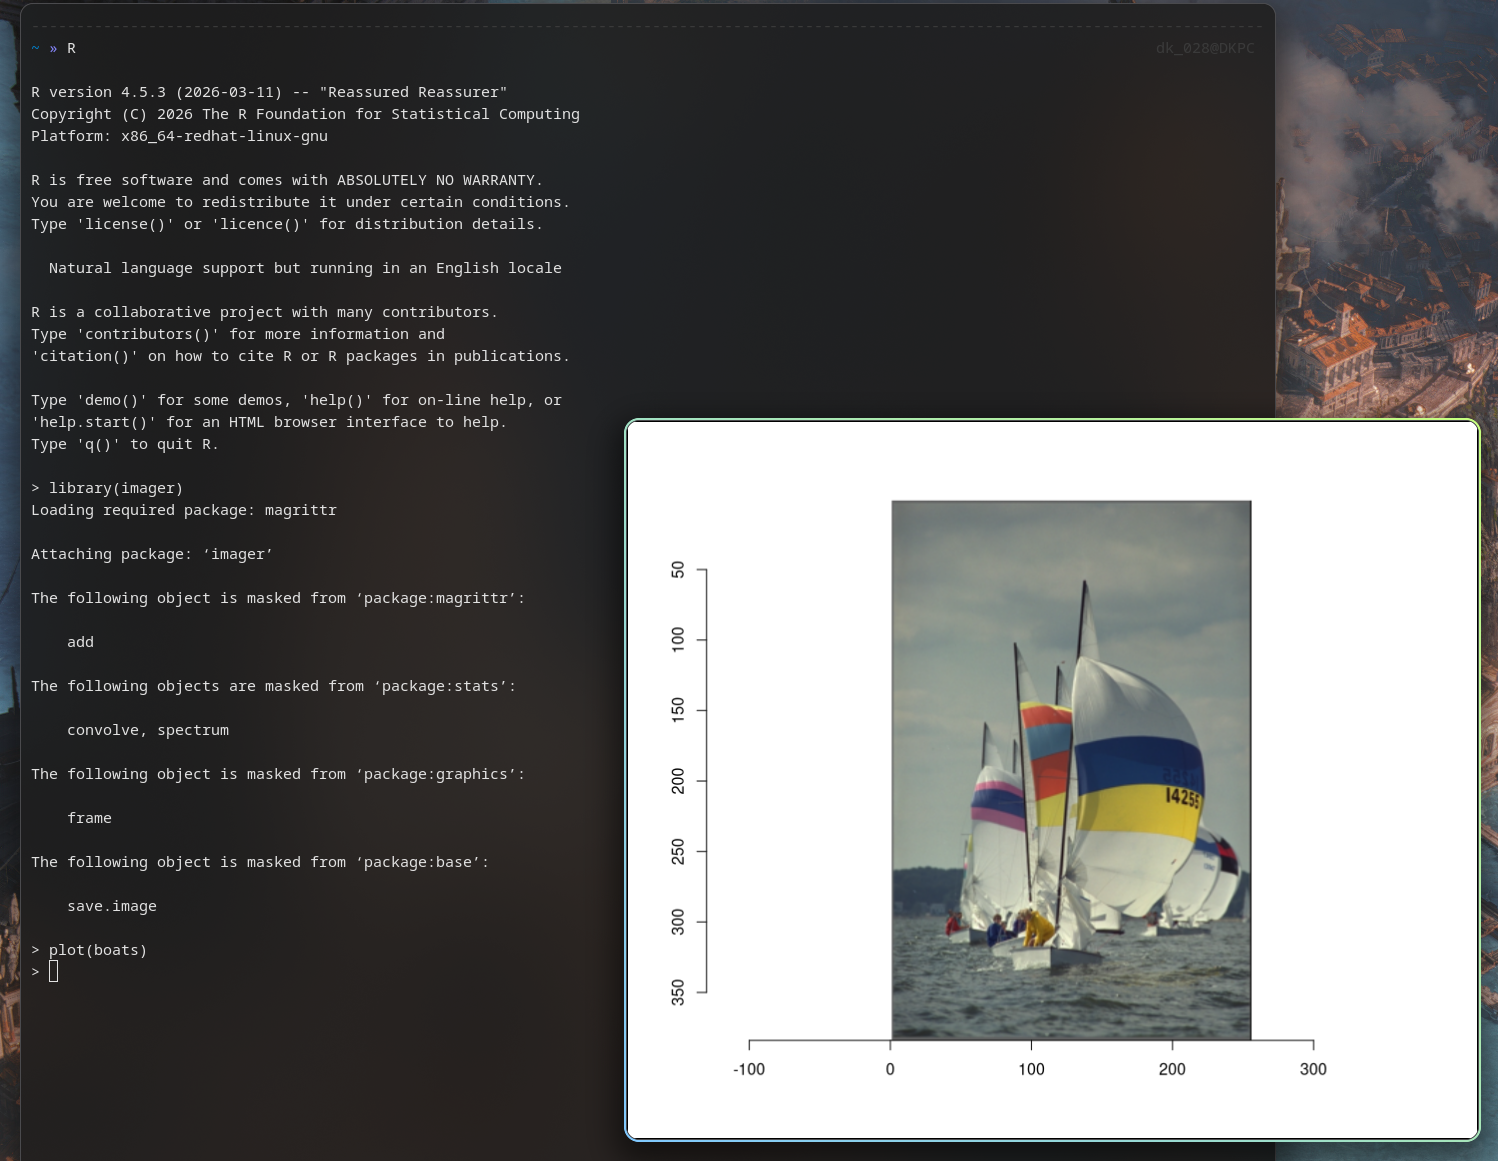
\includegraphics[width=0.9\linewidth]{images/screenshot.png}
    \caption{R における \texttt{plot(boats)} の実行結果}\label{fig:boats}
  \end{figure}
  \vspace{-1em}

  \subsubsection{説明}\label{subsubsec:task1-2-explanation}

  スクリーンショットより、\verb|imager| パッケージが正常にインストールされていることが確認できる。
  \verb|library(imager)| でパッケージを読み込み、\verb|plot(boats)| を実行することで、
  \verb|imager| に搭載されているサンプル画像「boats（舟）」がグラフィックウィンドウに表示された。

\subsection{課題２}\label{subsec:task2}

  複数の静止画像のフレームデータ（ビデオの１枚の画像）を作成して、時系列に並べて動画を制作。

  \begin{enumerate}[label = (\alph*)]
    \item フレームデータを動画制作ソフト（どのようなアプリでも良い）に取り込み、約10 秒間の動画を制作する。
    このとき、必要に応じて新たなフレーム画像を作成し、加除修正する。
    \item 完成した動画のフレーム周期（フレームレート）を変
    化して見え方（動きの滑らかさや面白さなど）を各自で評価する。
    \item 制作した作品は、動画ファイル（.mp4）にして保存する。
    このときファイル名は、「出席番号・氏名ー課題2」とすること。
  \end{enumerate}

  \subsubsection{結果}\label{subsubsec:task2-result}

  Aseprite を用いて、グラスに水が垂れて落ちる様子から個人のゲームスタジオのロゴに変身するアニメーションを制作した。
  フレーム数は32枚、1フレームあたりの表示時間は300\,msに設定し、合計再生時間は約9.6秒となった。
  完成した動画はmp4形式として保存した。

  \subsubsection{考察}\label{subsubsec:task2-explanation}

  1 フレームあたり 300\,ms（約 3.3\,fps）というフレームレートは、なめらかな映像として
  一般的に用いられる 24\,fps と比較して非常に低い。
  そのため、アニメーションの動作はコマ送り感が強く、動きのぎこちなさが目立った。
  一方、ロゴが現れる場面のように変化が少ないシーンでは低フレームレートでも違和感は小さかった。
  フレームレートを上げるためには、中間フレーム（トゥイーン）を追加してフレーム数を増やし、
  1 フレームあたりの表示時間を短くする必要がある。

\subsection{課題３}\label{subsec:task3}
  課題2で利用したフレーム（ビデオの１画像）データをR に取り込み、
  画像処理パッケージを利用した処理を実施してください。処理する画像は3枚。
  なお、実施する画像処理は、以下のpdf資料を参照して、各自が興味を持った処理を行うこと。

  \url{http://www.mi.u-tokyo.ac.jp/consortium2/pdf/4-6_literacy_level_note.pdf}

  \subsubsection{結果}\label{subsubsec:task3-result}

  アニメーション GIF（\texttt{glass-animation.gif}）からフレーム 5・15・25 を抽出し、
  各フレームにガウシアンフィルタ・鮮鋭化フィルタ・エッジ抽出フィルタを
  手動の行列演算で適用した。結果を図\ref{fig:task3-f05}〜\ref{fig:task3-f25}に示す。

  以下のスクリプトを実行した（組み込みフィルタ関数は使用しない）。

\lstinputlisting[language=R, caption={2次元畳み込みによる手動フィルタ処理}]{code/task3.R}

  % ── Frame 05 ──────────────────────────────────────────────────────────────
  \begin{figure}[htbp]
    \centering
    \begin{subfigure}[t]{0.3\linewidth}
      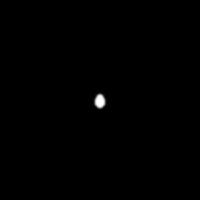
\includegraphics[width=\linewidth]{images/frame_05_blur.png}
      \caption{ガウシアンフィルタ}
    \end{subfigure}\hfill
    \begin{subfigure}[t]{0.3\linewidth}
      
\includegraphics[width=\linewidth]{images/frame_05_sharp.png}
      \caption{鮮鋭化フィルタ}
    \end{subfigure}\hfill
    \begin{subfigure}[t]{0.3\linewidth}
      
\includegraphics[width=\linewidth]{images/frame_05_edge.png}
      \caption{エッジ抽出}
    \end{subfigure}
    \caption{フレーム 05 への各フィルタ適用結果}
    \label{fig:task3-f05}
  \end{figure}

  % ── Frame 15 ──────────────────────────────────────────────────────────────
  \begin{figure}[htbp]
    \centering
    \begin{subfigure}[t]{0.3\linewidth}
      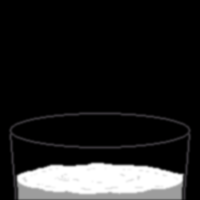
\includegraphics[width=\linewidth]{images/frame_15_blur.png}
      \caption{ガウシアンフィルタ}
    \end{subfigure}\hfill
    \begin{subfigure}[t]{0.3\linewidth}
      
\includegraphics[width=\linewidth]{images/frame_15_sharp.png}
      \caption{鮮鋭化フィルタ}
    \end{subfigure}\hfill
    \begin{subfigure}[t]{0.3\linewidth}
      
\includegraphics[width=\linewidth]{images/frame_15_edge.png}
      \caption{エッジ抽出}
    \end{subfigure}
    \caption{フレーム 15 への各フィルタ適用結果}
    \label{fig:task3-f15}
  \end{figure}

  % ── Frame 25 ──────────────────────────────────────────────────────────────
  \begin{figure}[htbp]
    \centering
    \begin{subfigure}[t]{0.3\linewidth}
      
\includegraphics[width=\linewidth]{images/frame_25_blur.png}
      \caption{ガウシアンフィルタ}
    \end{subfigure}\hfill
    \begin{subfigure}[t]{0.3\linewidth}
      
\includegraphics[width=\linewidth]{images/frame_25_sharp.png}
      \caption{鮮鋭化フィルタ}
    \end{subfigure}\hfill
    \begin{subfigure}[t]{0.3\linewidth}
      
\includegraphics[width=\linewidth]{images/frame_25_edge.png}
      \caption{エッジ抽出}
    \end{subfigure}
    \caption{フレーム 25 への各フィルタ適用結果}
    \label{fig:task3-f25}
  \end{figure}

  \subsubsection{考察}\label{subsubsec:task3-explanation}

  \vspace{8pt}
  \begin{description}[style=nextline, leftmargin=2em, topsep=6pt]
  \vspace{4pt}
    \item[ガウシアンフィルタ]
      5×5 のガウシアンカーネルを畳み込んだ結果、画像全体が平滑化され輪郭がぼやけた。
      これは周辺画素の加重平均を取ることでノイズ成分（高周波成分）が抑圧されるためである。
      PDFで説明された「画像のフィルタリング $f(x,y)$ に対しカーネル $h$ を畳み込む」操作に対応する。

  \vspace{4pt}
    \item[鮮鋭化フィルタ]
      中心係数 $+5$、上下左右が $-1$ の$3\times3$カーネルを適用した。
      これは元の画像からラプラシアン成分を引くアンシャープマスクと等価であり、
      エッジが強調されて細部がくっきりと見えた。
      ただし、高コントラスト境界の暗側に明るいハローが生じるのはこのカーネルの性質によるものである。

  \vspace{4pt}
    \item[ラプラシアンフィルタ（エッジ抽出）]
      中心係数 $-4$、隣接4画素が $+1$ のラプラシアンカーネルを適用し、
      輝度の2階微分を近似した。結果は輝度変化の大きい輪郭部分のみが白く浮かび上がり、
      均一な領域はほぼ黒になった。PDFで示されたエッジ強調の仕組みと一致する。

  \vspace{4pt}
    \item[実装の仕組み]
      \verb|imager| パッケージを画像の入出力のみに使用し、フィルタ処理は組み込み関数を一切用いない。
      \verb|load_img()| は \verb|load.image()| で読み込んだ \texttt{cimg} オブジェクトを
      通常の数値配列（グレースケール：2次元、カラー：3次元）に変換する。
      \verb|convolve2d()| はゼロパディング後に全画素についてカーネルとのアダマール積の和を
      計算する二重ループである。アニメーションの静止画はグレースケール画像とカラー画像の結合で作成したため、
      \verb|convolve_img()| は入力が2次元の場合にチャンネル次元を追加してから、
      各チャンネルに \verb|convolve2d()| を適用する。
      \verb|save_img()| は3次元配列をdepth次元を挿入した4次元 \texttt{cimg} に変換して保存する。
  \end{description}

\section{研究事項}\label{sec:research}
  \subsection{ビデオ映像の規格}\label{subsec:research1}

  ビデオ映像の規格は、解像度・フレームレート・走査方式の3つの要素で定義される。

  \begin{description}[style=nextline, leftmargin=2em, topsep=6pt]
  \vspace{4pt}
    \item[解像度]
      映像の精細さを表す画素数であり、水平×垂直の形式で示される。
      現在主流の規格は以下の通りである。
      \begin{itemize}
        \item \textbf{720p}（1280x720）：HD（ハイビジョン）。水平720ラインのプログレッシブ方式。
        \item \textbf{1080i / 1080p}（1920x1080）：フルHD（フルハイビジョン）。
              1080i はインターレース、1080p はプログレッシブ方式。
        \item \textbf{4K UHD}（3840x2160）：フルHDの4倍の画素数を持つ超高精細規格。
        \item \textbf{8K UHD}（7680x4320）：4Kのさらに4倍。スーパーハイビジョンとも呼ばれる。
      \end{itemize}
  \vspace{4pt}
    \item[フレームレート]
      1秒間に表示するフレーム（静止画）の枚数であり、fps（frames per second）で表す。
      映画は24fps、日本のテレビ放送（NTSC系）は約29.97fps、
      欧州（PAL系）は25fps が標準とされている。
      近年はゲームや配信向けに60fps、120fps、240fpsの規格も普及している。
  \vspace{4pt}
    \item[走査方式]
      映像をどのように画面に描画するかを定める方式であり、主に以下の2種類がある。
      \begin{itemize}
        \item \textbf{プログレッシブ（順次走査、p）}：全ラインを上から順に1フレームとして描画する。動きの速い映像に適している\cite{wikipedia_progressive}。
        \item \textbf{インターレース（飛び越し走査、i）}：奇数ラインと偶数ラインを交互に描画する。
              帯域幅を節約できるが、静止画でのちらつきが生じやすい\cite{wikipedia_interlace}。
      \end{itemize}
  \end{description}

  高精細度ビデオの仕様は1980年代に日本でNHKが1125ライン・30fpsのアナログ方式を開発したことに始まり、
  その後デジタル化が進み、現在はATSC・DVB・ISDBなどの国際規格が整備されている\cite{wikipedia_hd}。

  \subsection{フレーム周期と人間の視覚特性}\label{subsec:research2}

  映画はすべて静止画の連続であり、十分な速さで提示することで人間の観察者に
  なめらかな動きの印象を与える。Watson は、映像の時間サンプリングによって生じる
  アーティファクトの視認性を\textbf{可視性の窓（Window of Visibility）}という概念で
  定量的に説明するフレームワークを提案した\cite{watson2013}。

  \begin{description}[style=nextline, leftmargin=2em, topsep=6pt]
  \vspace{4pt}
    \item[時空間周波数と可視性の窓]
      映像信号はフーリエ変換によって時空間周波数領域で表現できる。
      人間の視覚系が感知できる範囲は、空間周波数の上限 $u_0$（約 32\,cycles/degree）と
      時間周波数の上限 $w_0$（約 32\,Hz）によって菱形状に区画される可視性の窓として
      近似される。時間サンプリング（フレーム化）によって生じるスペクトル複製が
      この窓の外に収まる限り、映像はなめらかに見える。
  \vspace{4pt}
    \item[臨界フリッカー周波数（CFF）と輝度]
      時間方向の感度上限 $w_0$ は臨界フリッカー周波数とも呼ばれ、
      輝度に依存して増加する（Ferry-Porter の法則）。
      デジタルシネマスクリーンの高輝度基準（48\,cd/m\textsuperscript{2}）では
      CFF は約 60\,Hz に達し、窓の大きさ自体が変化する。
  \vspace{4pt}
    \item[臨界フレームレートと運動速度]
      被写体が画面上を速度 $r$（degree/sec）で移動するとき、
      アーティファクトが可視性の窓に侵入しない最低フレームレート $w_c$ は次式で与えられる：
      \begin{equation}
        w_c =
        \begin{cases}
          w_0       & (r \leq r_0) \\
          r \cdot u_0 & (r > r_0)
        \end{cases}
      \end{equation}
      ここで $r_0 = w_0/u_0$（約 1\,degree/sec）は臨界速度である。
      動きが遅い場合（$r \leq r_0$）は $w_c = w_0$（約 32\,Hz）で十分だが、
      動きが速くなるほど必要なフレームレートは線形に増加し、
      4\,degree/sec では理論上 120\,Hz が必要になる場合もある。
  \vspace{4pt}
    \item[残像との違い]
      動画のなめらかさは古くから残像（persistence of vision）によって
      説明されることが多かったが、Watson はこの概念が定量的な予測に
      つながらないと指摘している。可視性の窓モデルは、フリッカー・多重像・
      モーションブラーといった異なる種類のアーティファクトを統一的に
      説明でき、フレームレートや露光時間（シャッター角度）などの
      パラメータ選択に科学的根拠を提供する。
  \end{description}

\section{感想}\label{sec:impressions}

今回の実験では、アニメーション制作と画像処理という二つの側面から、映像の仕組みを実践的に学ぶことができた。

アニメーション制作において、Aseprite を使用したが、以前は自作ゲームのために簡単なアニメーションを
制作した経験があったものの、それから約2年が経過しており、操作方法をほとんど忘れてしまっていた。
そのため、今回は改めてツールの使い方を学び直す必要があり、基本操作を一から確認しながら作業を進めた。

プログラミングについては、普段はバックエンド開発でC・C++・Rustといったシステムプログラミング言語を
主に使用しているため、Rのような統計・データ処理向け言語は新鮮な体験であった。
画像をそのまま数値行列として扱い、フィルタ処理を行列演算として表現できる点は、
数学的な直感と対応しやすく、Rの設計思想の合理性を感じた。
普段とは異なるパラダイムの言語を学ぶことは、プログラミングに対する理解を広げる良い機会となった。

\addcontentsline{toc}{section}{参考文献}
\begin{thebibliography}{9}
  \bibitem{wikipedia_hd}
    Wikipedia,
    ``高精細度ビデオ'',
    \url{https://ja.wikipedia.org/wiki/高精細度ビデオ},
    （参照 \today）
  \bibitem{wikipedia_progressive}
    Wikipedia,
    ``プログレッシブ・スキャン'',
    \url{https://ja.wikipedia.org/wiki/プログレッシブ・スキャン},
    （参照 \today）
  \bibitem{wikipedia_interlace}
    Wikipedia,
    ``インターレース'',
    \url{https://ja.wikipedia.org/wiki/インターレース},
    （参照 \today）
  \bibitem{watson2013}
    A. B. Watson,
    ``High Frame Rates and Human Vision: A View Through the Window of Visibility'',
    \textit{SMPTE Motion Imaging Journal}, vol.~122, pp.~18--32, 2013,
    doi: 10.5594/j18266.
\end{thebibliography}


\end{document}
